\documentclass[a4paper,UTF8]{ctexart}

\usepackage{amsmath, amsthm, amssymb, amsfonts, hyperref, mathrsfs}%美国数学学会的包+?
\usepackage{geometry} %控制界面
\usepackage{bookmark}
\usepackage{fancyhdr} % header & footer
\usepackage{appendix} % 附录
\usepackage{tikz} %作图
\usepackage{graphicx} %插入图片的宏包
\usepackage{float} %设置图片浮动位置的宏包
\usepackage{subfigure} %插入多图时用子图显示的宏包
\usepackage{listings} %引用代码
\usepackage{physics,mathtools} %物理数学工具
\usepackage{comment}
\usepackage{framed}
\geometry{top=2.5cm,bottom=2.5cm,left=2.5cm,right=2.5cm} % 布局要求
\pagestyle{fancy} % fancy分格
\fancyhf{} % 清除所有页眉页脚
\renewcommand\headrulewidth{0.6pt}
\renewcommand\footrulewidth{0.6pt}
\lhead{何金铭 PB21020660$\mid$座位号:1}
\chead{光纤传感器实验报告}
\rhead{\thepage}
\lfoot{2022.11.10}
\rfoot{USTC}
%\bibliographystyle{plain} % 引用样式
\everymath{\displaystyle} % display
%============================================================

\begin{document}

\begin{center}
    \textbf{\Large 光纤传感器实验报告}
    \par \text{\large 何金铭 PB21020660}
\end{center}

\section{实验待研究部分}

\begin{enumerate}
    \item 透射型和反射型光纤位移传感器是如何工作的?
    \item 微弯光纤位移传感器的原理和工作特点如何?
\end{enumerate}

\section{实验原理}

\subsection{透射式横(纵)向光纤位移传感}

透射式光纤位移传感是一种强度型光纤传感,实验通过改变两透射多模光纤
出光芯径的相对位置(横向或者纵向)观测传输功率的变化,从而绘制功率随横
向或纵向位移的关系曲线。

如上式可见当光线本身参数一定时,出射光场光强与偏离光纤轴线距离和
与发射端面的距离都有关。如果接受光纤采用与发射光纤同种光纤时,所接收到
的光强可表示为:

\begin{equation}
    I(r,z) = \iint_{\Sigma} \frac{I_0}{\pi \omega^2(z)} \exp{- \frac{r^2}{\omega^2(z)}} \,ds 
\end{equation}

(1)式中$\omega(z) = \sigma a_0 \left[1+\xi (\frac{z}{a})^{\frac{3}{2}}\right]$这里,S 为接收光面,即纤芯端面。


\begin{comment}
当
z 固定时,得到的是横向位移传感特性函数,当 r 取定时(如 r=0),则可得到纵
向位移传感特性函数。

调制处的光纤端面为平面,通常发射光纤不动,而接收光纤可以做横向位移,
纵向位移。这样,接收光纤的输出光强被其位移调制。这里采用发射光纤不动,
接收光纤移动的办法,实现光纤被横向位移和纵向位移调制。
\end{comment}


\begin{figure}[H]
    \centering
    \begin{minipage}[b]{0.9\textwidth}
        \centering
        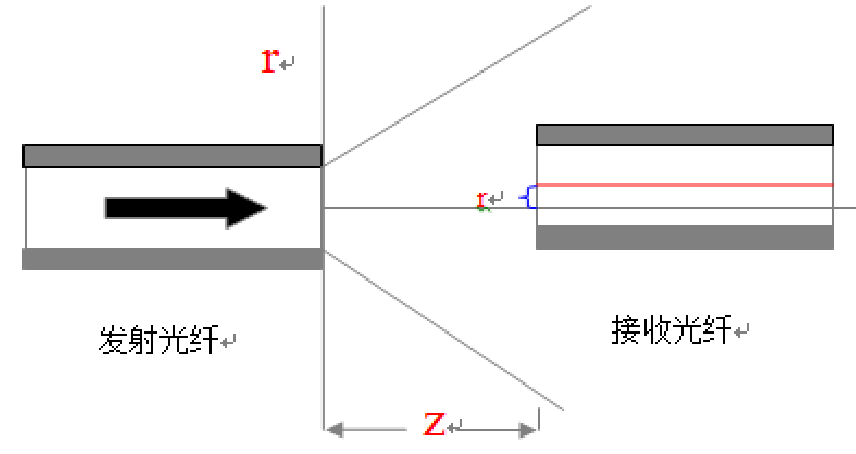
\includegraphics[width=0.5\textwidth]{./1.png}
        \caption{光纤位移传感器示意图}
    \end{minipage}
\end{figure}

\subsection{反射式光纤位移传感}

反射式光纤传感实验的光纤探头 A 由两根光纤组成,一根用于发射光,一根
用于接收反射回来的光,R 是反射材料的反射率。由发射光纤发出的光照射到反
射材料上,通过检测反射光的强度变化,就能测出反射体的位移。

在反射式光纤位移传感器中,探头结构中发射光纤与反射光纤使用同种光纤
时,接收到的光强可表示为:

\begin{equation}
    I(r,x) = \iint_{\Sigma} \frac{I_0}{\pi \omega^2(x)} \exp{- \frac{r^2}{\omega^2(x)}} \,ds 
\end{equation}

(1)式中$\omega(x) = \sigma a_0 \left[1+\xi (\frac{x}{a})^{\frac{3}{2}}\right]$这里,S 为接收光面,即纤芯端面。

\begin{figure}[H]
    \centering
    \begin{minipage}[b]{0.9\textwidth}
        \centering
        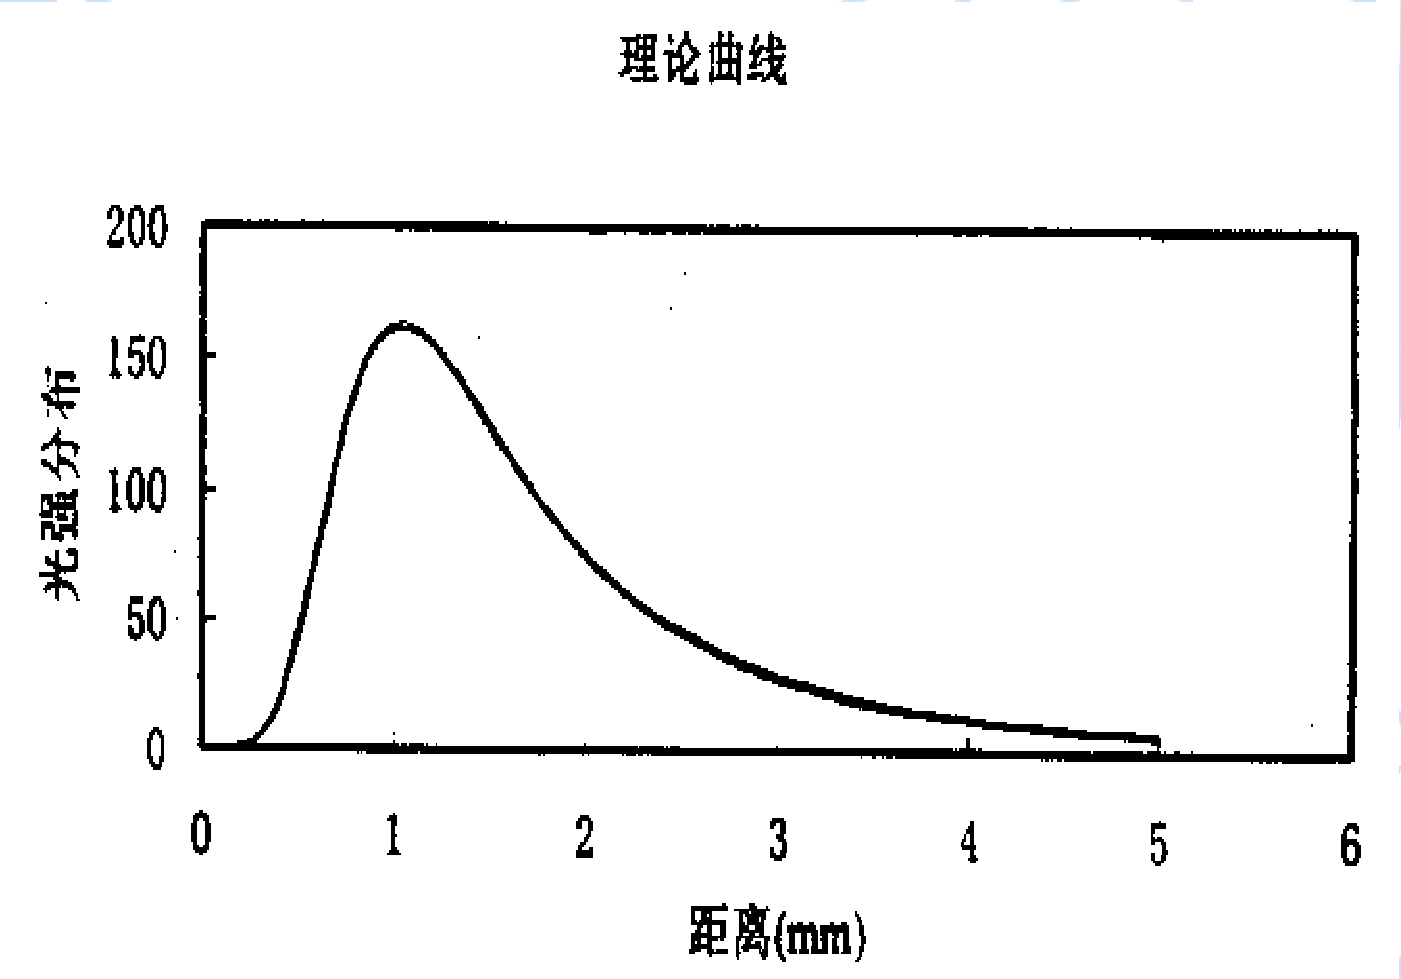
\includegraphics[width=0.5\textwidth]{./2.png}
        \caption{反射式调制特性曲线}
    \end{minipage}
\end{figure}

\subsection{微弯光纤位移传感器}

微弯型光纤传感器的原理结构如下图(4)所示。当光纤发生弯曲时,由于其
全反射条件被破坏,纤芯中传播的某些模式光束进入包层,造成光纤中的能量损
耗。

为了扩大这种效应,我们把光纤夹持在一个周期波长为
$\Lambda$的梳妆结构中。当
梳妆结构(变形器)受力时,光纤的弯曲情况将发生变化,于是纤芯中跑到包层
中的光能(即损耗)也将发生变化。

\begin{figure}[H]
    \centering
    \begin{minipage}[b]{0.9\textwidth}
        \centering
        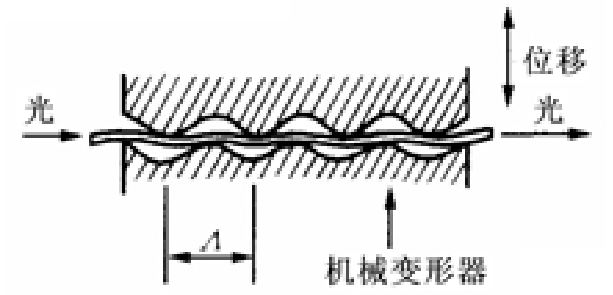
\includegraphics[width=0.5\textwidth]{./3.png}
        \caption{微弯位移传感器示意图}
    \end{minipage}
\end{figure}

\section{实验仪器}

光纤输出 650nm 半导体激光器、反射式传感用光纤、透射式传
感用光纤、微弯型光纤、光纤功率计、反射镜、控制电源
、微调位移台、承托位移台。

\section{实验数据及处理}

\subsection{光纤位移传感实验}

\begin{table}[H]
    \centering
    \begin{tabular}{|c|c|c|c|c|c|c|c|c|}
    \hline
        纵向/$mm$ & $x_0 = 15.500$ & $+0.05 \times 1$ & 2 & 3 & 4 & 5 & 6 & 7 \\ \hline
        功率/$\mu W$ & 324.3 & 302.3 & 267.0 & 223.7 & 194.5 & 166.0 & 147.4 & 129.8 \\ \hline
        纵向/$mm$ & 8 & 9 & 10 & 11 & 12 & 13 & 14 & 15 \\ \hline
        功率/$\mu W$ & 115.2 & 104.1 & 95.41 & 88.18 & 80.54 & 75.05 & 69.04 & 63.12 \\ \hline
        纵向/$mm$ & 16 & 17 & 18 & 19 & 20 & 21 & 22 & 23 \\ \hline
        功率/$\mu W$ & 59.05 & 55.52 & 51.97 & 48.40 & 43.49 & 39.20 & 35.41 & 31.76 \\ \hline
        纵向/$mm$ & 24 & ~ & ~ & ~ & ~ & ~ & ~ & ~ \\ \hline
        功率/$\mu W$ & 29.54 & ~ & ~ & ~ & ~ & ~ & ~ & ~ \\ \hline
    \end{tabular}
    \caption{透射式位移传感功率-纵向位置关系原始数据}
\end{table}

\begin{figure}[H]
    \centering
    \begin{minipage}[b]{0.9\textwidth}
        \centering
        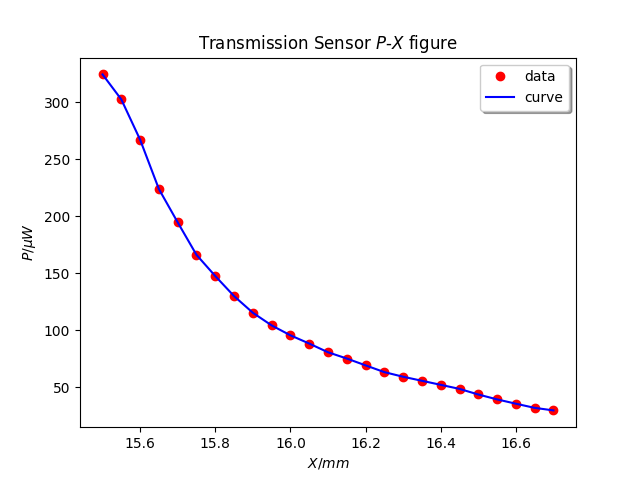
\includegraphics[width=0.7\textwidth]{./one_x.png}
        \caption{透射式位移传感功率-纵向位置关系}
    \end{minipage}
\end{figure}

{\bfseries 变化规律}

\begin{enumerate}
    \item 光功率整体趋势随纵向位移的增大而下降。
    \item 且光功率的下降速度随纵向位置的加大而下降。
\end{enumerate}

{\bfseries 与理论比较}

与公式(1)比较可得:当$r=0$时,光强$I(r,z)$从某个值开始是一个单减函数,且下降速度随纵向位置$z$的增大而下降,符合理论分析。

\begin{table}[H]
    \centering
    \begin{tabular}{|c|c|c|c|c|c|c|c|c|}
    \hline
        横向/$mm$ & $y_0 = 12.250$ & $+0.01 \times 1$ & 2 & 3 & 4 & 5 & 6 & 7 \\ \hline
        功率/$\mu W$ & 335.5 & 302.1 & 235.3 & 112.6 & 50.10 & 16.72 & 1.674 & $87.71 \times 10^{-3}$ \\ \hline
        横向/$mm$ & 8 & 9 & 10 & 11 & 12 & 13 & 14 & 15 \\ \hline
        功率/$n W$ & 67.10 & 48.95 & 43.13 & 33.27 & 21.05 & 9.120 & 8.250 & 7.974 \\ \hline
        横向/$mm$ & -1 & -2 & -3 & -4 & -5 & -6 & -7 & -8 \\ \hline
        功率/$\mu W$ & 288.7 & 183.9 & 112.0 & 49.12 & 15.36 & 3.175 & $83.68 \times 10^{-3}$ & $ 57.64\times 10^{-3}$ \\ \hline
        横向/$mm$ & -9 & -10 & -11 & -12 & -13 & -14 & -15 & ~ \\ \hline
        功率/$n W$ & 54.11 & 49.42 & 42.02 & 15.43 & 8.107 & 7.74 & 6.230 & ~ \\ \hline
    \end{tabular}
    \caption{透射式位移传感功率-横向位置关系原始数据}
\end{table}

\begin{figure}[H]
    \centering
    \begin{minipage}[b]{0.9\textwidth}
        \centering
        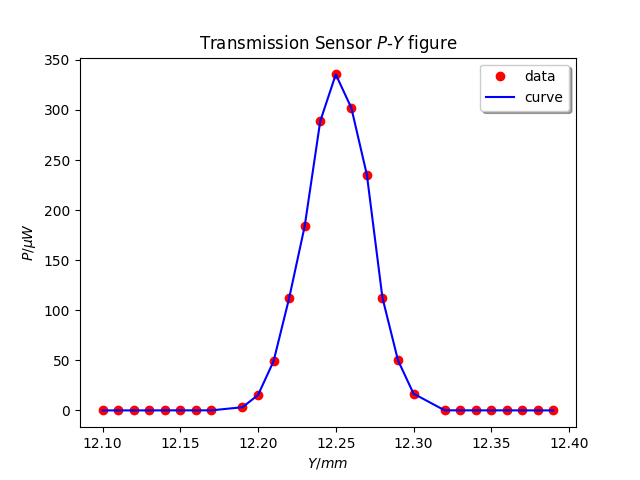
\includegraphics[width=0.7\textwidth]{./one_y.png}
        \caption{透射式位移传感功率-横向位置关系}
    \end{minipage}
\end{figure}

{\bfseries 变化规律}

\begin{enumerate}
    \item 光功率曲线大致关于光纤中心$y=12.250mm$的位置对称,呈现偶函数的形式。
    \item $y > 0$时,光功率$P$随$y$增加而递减;$y < 0$时,光功率$P$随$y$增加而递增。
    \item 且$y > 0$时,光功率的下降速度随着横向距离的增大而下降;$y<0$时,光功率的特征由偶函数的性质可容易给出。
\end{enumerate}

{\bfseries 与理论比较}

与公式(1)比较可得:当$z$固定时,光强$I(r,z)$是一个偶函数,于$r$正半轴单减,且下降速度随纵向位置$z$的增大而下降,呈现钟形,符合理论分析。

\subsection{反射式位移传感实验}

\begin{table}[H]
    \centering
    \begin{tabular}{|c|c|c|c|c|c|c|c|c|}
    \hline
        纵向/$mm$ & $x_0 = 3.050$ & $+0.05 \times 1$ & 2 & 3 & 4 & 5 & 6 & 7 \\ \hline
        功率/$\mu W$ & 1.181 & 6.330 & 17.36 & 34.10 & 54.31 & 76.58 & 100.5 & 122.5 \\ \hline
        纵向/$mm$ & 8 & 9 & 10 & 11 & 12 & 13 & 14 & 15 \\ \hline
        功率/$\mu W$ & 145.5 & 167.5 & 189.1 & 205.8 & 222.4 & 236.5 & 250.2 & 261.7 \\ \hline
        纵向/$mm$ & 16 & 17 & 18 & 19 & 20 & 21 & 22 & 23 \\ \hline
        功率/$\mu W$ & 273.1 & 281.3 & 288.7 & 295.0 & 303.0 & 306.3 & 311.5 & 316.0 \\ \hline
        纵向/$mm$ & 24 & 25 & 26 & 27 & 28 & 29 & 30 & 31 \\ \hline
        功率/$\mu W$ & 319.5 & 321.1 & 323.7 & 324.3 & 324.5 & 324.8 & 323.1 & 322.6 \\ \hline
        纵向/$mm$ & 32 & 33 & 34 & 35 & 36 & 37 & 38 & 39 \\ \hline
        功率/$\mu W$ & 320.1 & 317.7 & 315.0 & 312.5 & 308.4 & 304.3 & 300.4 & 296.5 \\ \hline
        纵向/$mm$ & 40 & 41 & 42 & 43 & 44 & 45 & 46 & 47 \\ \hline
        功率/$\mu W$ & 290.8 & 285.7 & 281.6 & 277.1 & 271.8 & 266.1 & 261.9 & 256.5 \\ \hline
        纵向/$mm$ & 48 & 49 & 50 & 51 & 52 & 53 & 54 & 55 \\ \hline
        功率/$\mu W$ & 251.8 & 245.8 & 241.4 & 236.6 & 230..8 & 226.5 & 221.3 & 216.6 \\ \hline
        纵向/$mm$ & 56 & 57 & 58 & 59 & 60 & ~ & ~ & ~ \\ \hline
        功率/$\mu W$ & 213.7 & 209.9 & 203.8 & 201.5 & 196.6 & ~ & ~ & ~ \\ \hline
    \end{tabular}
    \caption{反射式位移传感功率-纵向位置关系原始数据}
\end{table}

\begin{figure}[H]
    \centering
    \begin{minipage}[b]{0.9\textwidth}
        \centering
        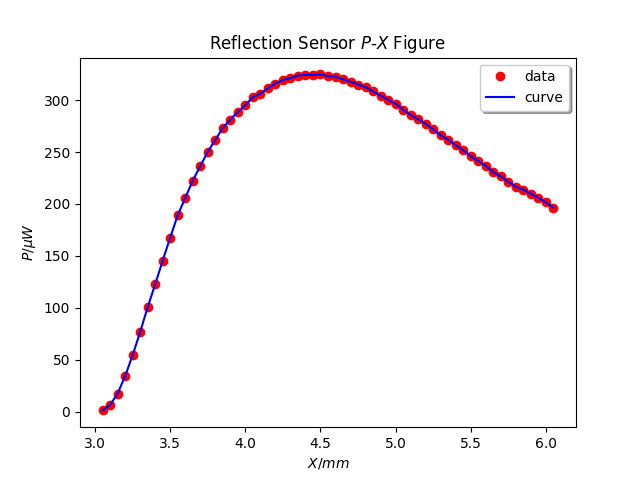
\includegraphics[width=0.7\textwidth]{./two.png}
        \caption{反射式位移传感功率-纵向位置关系}
    \end{minipage}
\end{figure}

{\bfseries 变化规律}

\begin{enumerate}
    \item 光功率曲线的随着纵向位置$x$的增大而降低。
    \item 光功率于纵向距离$x=4.500mm$处达到最大值。
    \item 且光功率曲线不对称,于曲线峰值的右侧的光功率上升的速度更快,于曲线峰值的左侧光功率下降的速度更慢。
\end{enumerate}

{\bfseries 与理论比较}

与公式(2)比较可得:当$r$固定时,光强$I(r,x)$是一个先增后减的函数,存在一个极大值,且于极大值右侧下降速度随纵向位置$z$的增大而下降,符合理论分析。

\subsection{微弯位移传感实验}

\begin{table}[H]
    \centering
    \begin{tabular}{|c|c|c|c|c|c|c|c|c|}
    \hline
        纵向/$mm$ & $x_0 = 18.500$ & $+0.05 \times 1$ & 2 & 3 & 4 & 5 & 6 & 7 \\ \hline
        功率/$\mu W$ & 4.916 & 4.907 & 4.893 & 4.879 & 4.854 & 4.831 & 4.804 & 4.818 \\ \hline
        纵向/$mm$ & 8 & 9 & 10 & 11 & 12 & 13 & 14 & 15 \\ \hline
        功率/$\mu W$ & 4.874 & 4.856 & 4.806 & 4.808 & 4.737 & 4.563 & 4.524 & 4.559 \\ \hline
        纵向/$mm$ & 16 & 17 & 18 & 19 & 20 & 21 & 22 & 23 \\ \hline
        功率/$\mu W$ & 4.560 & 4.549 & 4.462 & 4.437 & 4.481 & 4.490 & 4.632 & 4.573 \\ \hline
        纵向/$mm$ & 24 & 25 & 26 &  &  &  &  &  \\ \hline
        功率/$\mu W$ & 4.443 & 4.426 & 4.479 &  &  &  &  &  \\ \hline
    \end{tabular}
    \caption{微弯位移传感功率-纵向位置关系原始数据}
\end{table}

\begin{figure}[H]
    \centering
    \begin{minipage}[b]{0.9\textwidth}
        \centering
        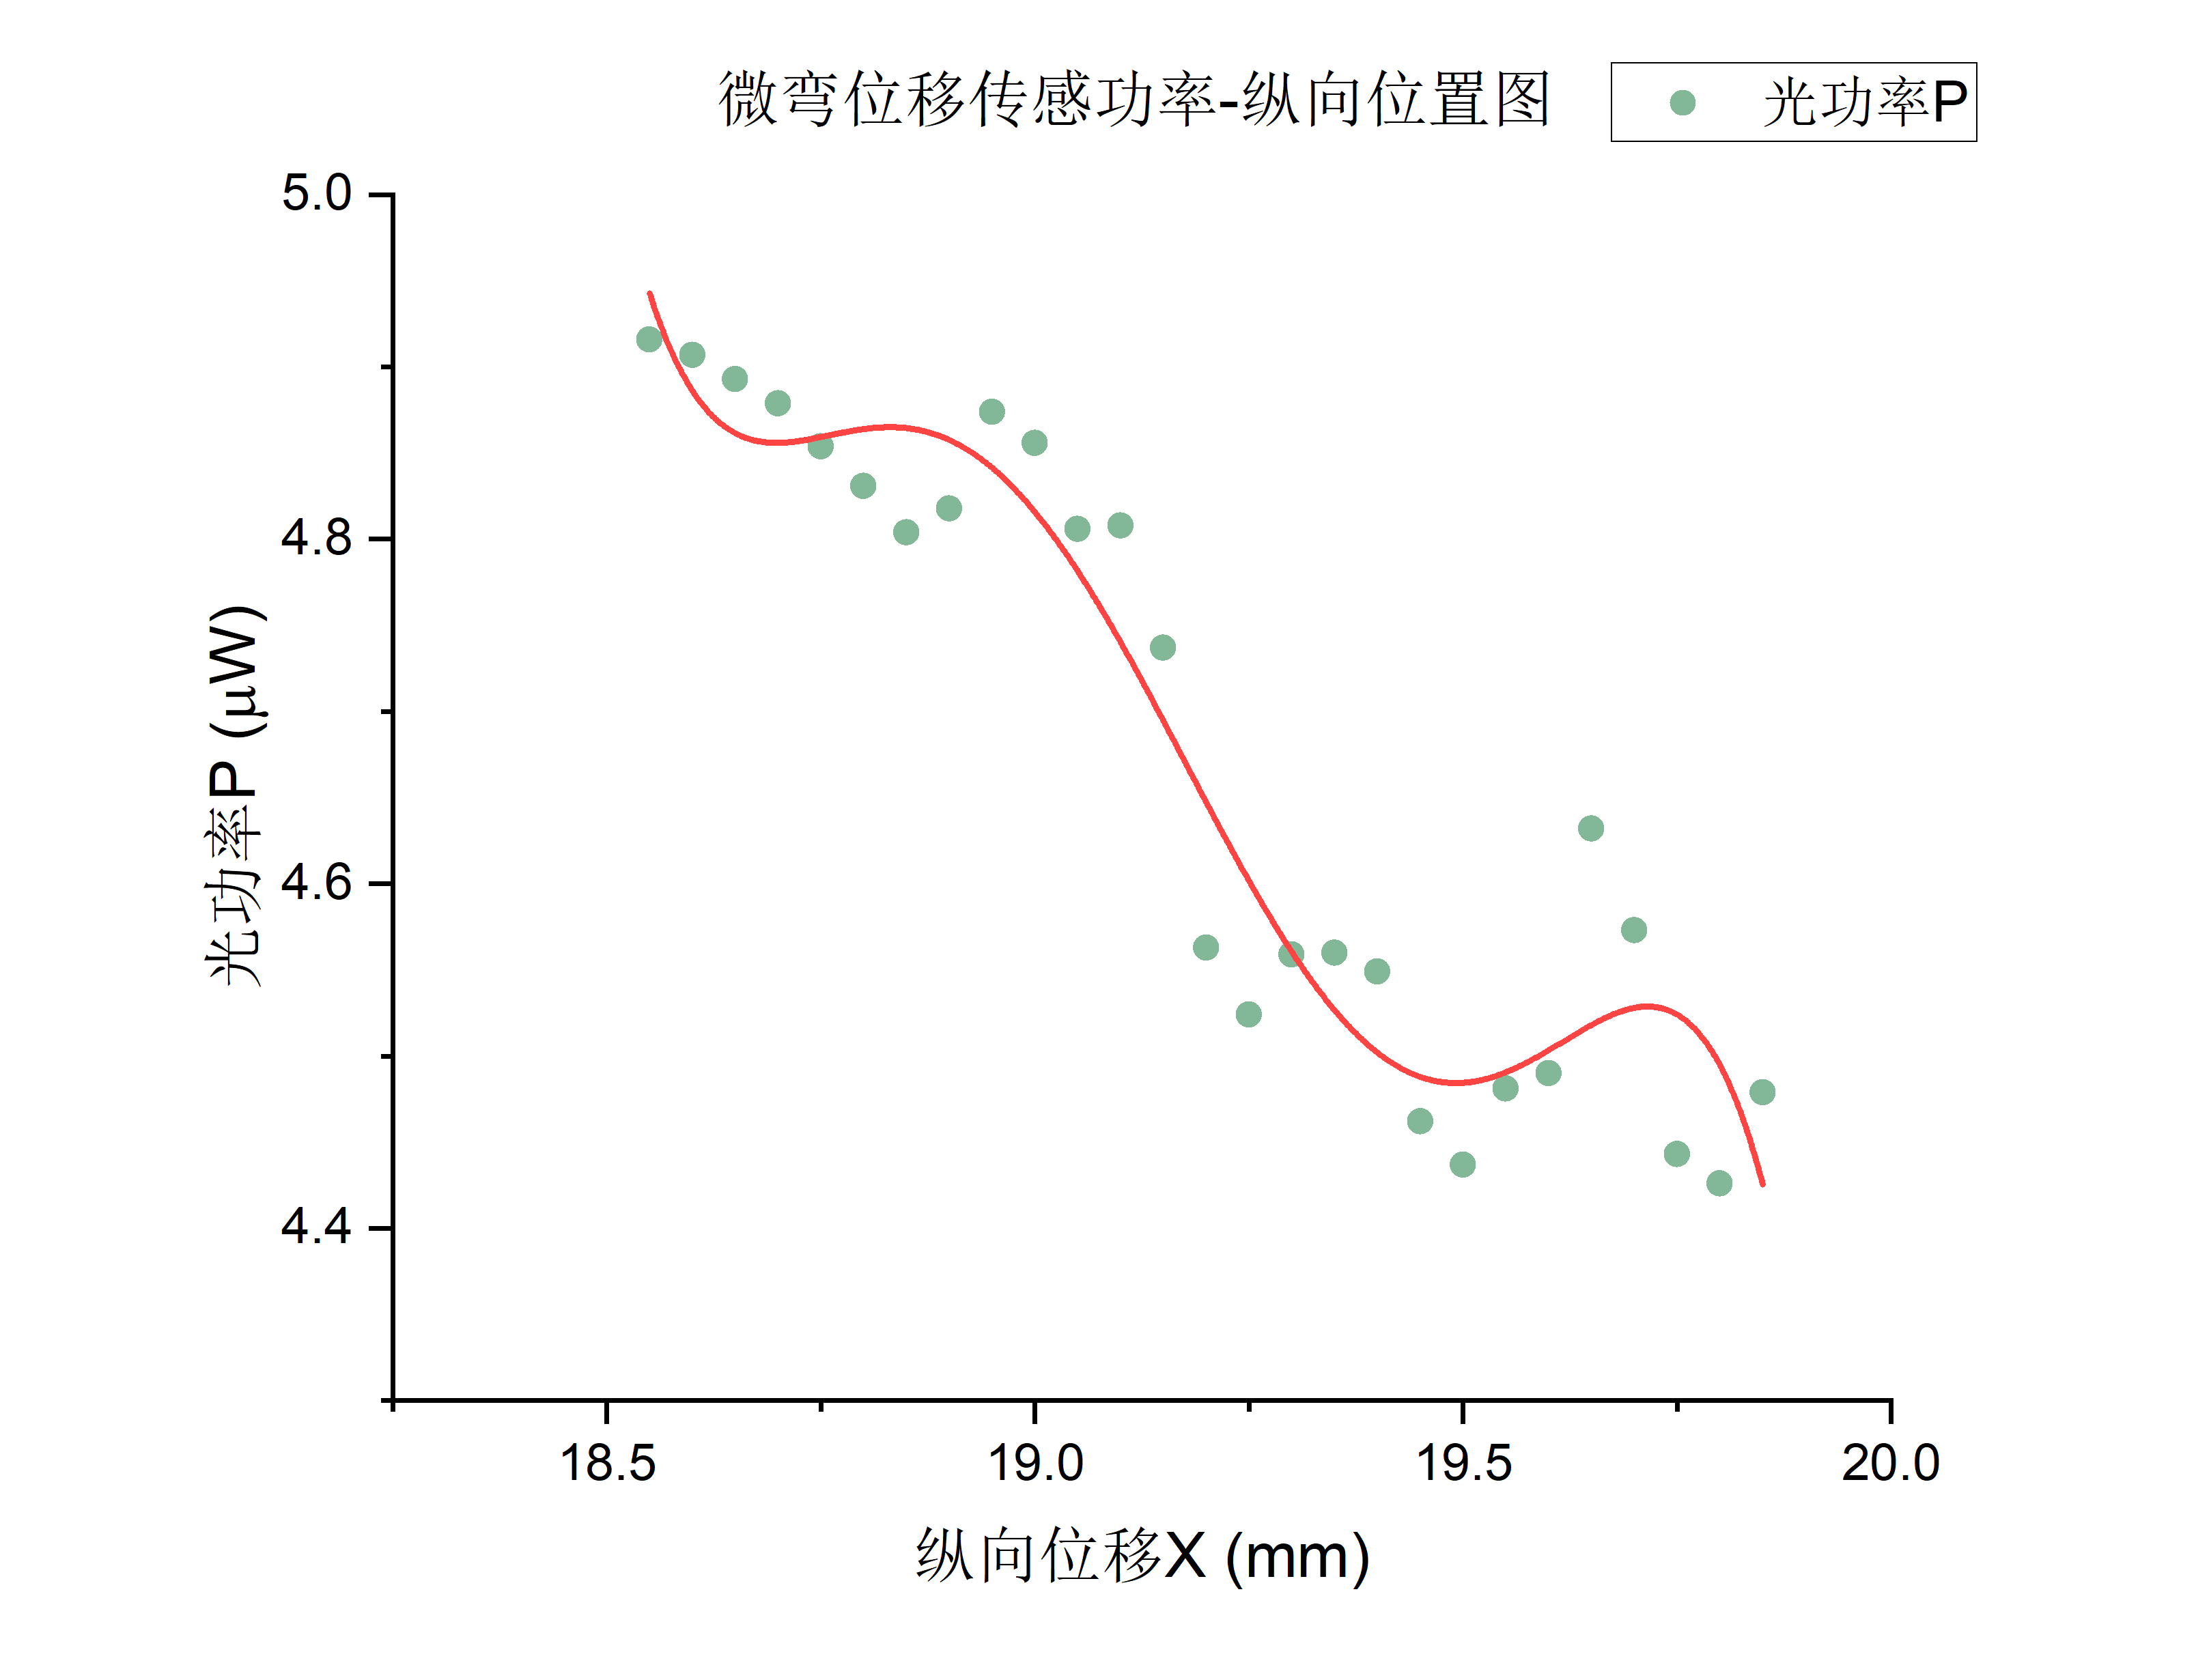
\includegraphics[width=0.7\textwidth]{./Graph6.png}
        \caption{微弯位移传感功率-纵向位置关系}
    \end{minipage}
\end{figure}

{\bfseries 变化规律}

\begin{enumerate}
    \item 光功率曲线整体呈现下降趋势。
    \item 光功率的曲线会有部分曲折的部分。
\end{enumerate}

{\bfseries 与理论比较}

由理论可知,当纵向位移加大的时候,光功率的整体曲线应该是呈下降趋势的;光功率曲线也可能有所起伏,但此处的起伏过大,应该认为是外界干扰所致。

\section{实验总结和误差分析}

\subsection{实验收获}

第一次做和光纤相关的实验,在完成实验之后对不同光纤的工作原理、光纤实验中常用的一些实验器材、光纤实验技巧等均有了一些了解。

\begin{enumerate}
    \item 了解了光纤的工作原理,也学习了不同光纤的形态、工作原理以及适用的工作环境。
    \item 在了解了光纤的原理之后,可以对实验有更好的把握,更加利于对实验误差的排查。
    \item 在实验的过程中,逐渐掌握了在光纤实验排除实验误差的方法。
    \item 学习了光纤的具体使用方法。
\end{enumerate}

\subsection{出现的问题}

\begin{enumerate}
    \item 在做光纤位移传感实验一开始的时候发现光功率计的示数一直在大幅度跳动,排查了许久的错误,最后发现是有一根光纤发生了漏光现象。
    最终的解决方法是:换用了一根其他的光纤。
    \item 在微弯位移传感实验中,由于光纤极为容易漏光,所以外界的微小扰动就会影响光功率的读数。并且由于实验时间不够,所以动作幅度略微偏大,导致测得的曲线跳动不定。
\end{enumerate}

\subsection{误差分析}

\subsubsection{系统误差}

\begin{enumerate}
    \item 由于光纤中轴线与光纤中轴线无法严格对齐的系统误差。
    \item 由于光纤中轴线与镜面无法严格垂直的系统误差。
    \item 在微弯光纤传感器中,两个用于变形的装置没有完全垂直对齐,导致弯曲不均匀;且初始的光纤未完全拉直,也会使曲线一开始有明显的震荡。
    \item 在三个实验中,光纤均存在漏光现象,所以对光功率整体有一个下降的系统误差。
\end{enumerate}

\end{document}